%
\documentclass{beamer}
\usepackage{caption}
\usepackage{subcaption}
\usepackage{../../arbenson-math}
\usepackage{graphics}

\graphicspath{{./figures/}}
\usetheme{boxes}
\usecolortheme{seahorse}

\AtBeginSection[]
{
  \begin{frame}<beamer>
    \frametitle{\thesection}
    \tableofcontents[currentsection]
  \end{frame}
}

\title{CME 193: Introduction to Scientific Python \\
Lecture 4: NumPy and SciPy}
\author{
Dan Frank \\
\vspace{0.1in}
Institute for Computational and Mathematical Engineering (ICME)}
\date{January 21, 2014}
\begin{document}

\maketitle

\section{NumPy}

\begin{frame}
\frametitle{What is NumPy?}

Wikipedia: NumPy is an extension to the Python programming language, adding support for large, multi-dimensional arrays and matrices, along with a large library of high-level mathematical functions to operate on these arrays.

\begin{itemize}
\setlength{\itemsep}{0.1in}
\item{At the core of the NumPy package, is the \textit{ndarray} object which encapsulates n-dimensional arrays of homogeneous data. 
}
\item{Many operations performed using \textit{ndarray} objects execute in compiled code for performance}
\item{The standard mathematical and scientific packages in Python use NumPy arrays}
\end{itemize}
\end{frame}

\begin{frame}
\frametitle{Array Creation}
Several ways to create arrays...
\lstset{basicstyle=\scriptsize}
\codeblock{code/array_creation.py}
\end{frame}

\begin{frame}
\frametitle{Array IO}
\lstset{basicstyle=\small}
\codeblock{code/array_io.py}
Other options control data types, delimiters, comments, headers, etc.
See documentation, especially "See Also". And for matlab \texttt{scipy.io.matlab}
\end{frame}

\begin{frame}
\frametitle{Array Attribtues}
Arrays are objects and so have attributes and methods.
\codeblock{code/array_attributes.py}
And many others. Explore in documentation or with TAB complete in ipython.
\end{frame}


\begin{frame}
\frametitle{Array Slicing and Indexing}
Similar to lists but a few new ways to select
\lstset{basicstyle=\scriptsize}
\codeblock{code/array_slice.py}
\end{frame}

\begin{frame}
\frametitle{Array Slicing and Indexing}
Different indexing can be very powerful, used for extraction and setting of data.
\lstset{basicstyle=\scriptsize}
\codeblock{code/array_bool.py}
\end{frame}

\begin{frame}
\frametitle{Array Axes}
Arrays are organized by their axes, the first being row, then column, ...
\lstset{basicstyle=\scriptsize}
\codeblock{code/array_axes.py}
Many functions in NumPy and SciPy are created to operate along axes
\end{frame}


\begin{frame}
\frametitle{Array Operations \& ufuncs}
Default behavior is elementwise 
\lstset{basicstyle=\scriptsize}
\codeblock{code/array_operations.py}
\end{frame}

\begin{frame}
\frametitle{Array Broadcasting \& Vectorization}
Broadcasting allows us to operate on arrays of different shapes by reusing smaller arrays when possible. This allows us to write more efficient and readable code (with fewer for loops).
\codeblock{code/array_broadcasting.py}
\end{frame}

\begin{frame}
\frametitle{Array Broadcasting Rules}
When operating on two arrays, NumPy compares their shapes element-wise. It starts with the trailing dimensions, and works its way forward. Two dimensions are compatible when
\begin{enumerate}
\item they are equal, or
\item one of them is 1
\end{enumerate}
If these conditions are not met, a ValueError: frames are not aligned exception is thrown, indicating that the arrays have incompatible shapes. The size of the resulting array is the maximum size along each dimension of the input arrays.
\end{frame}

\begin{frame}
\frametitle{Array Broadcasting Example}
\begin{figure}
    \centering
	\begin{subfigure}[b]{\textwidth}
	\centering
	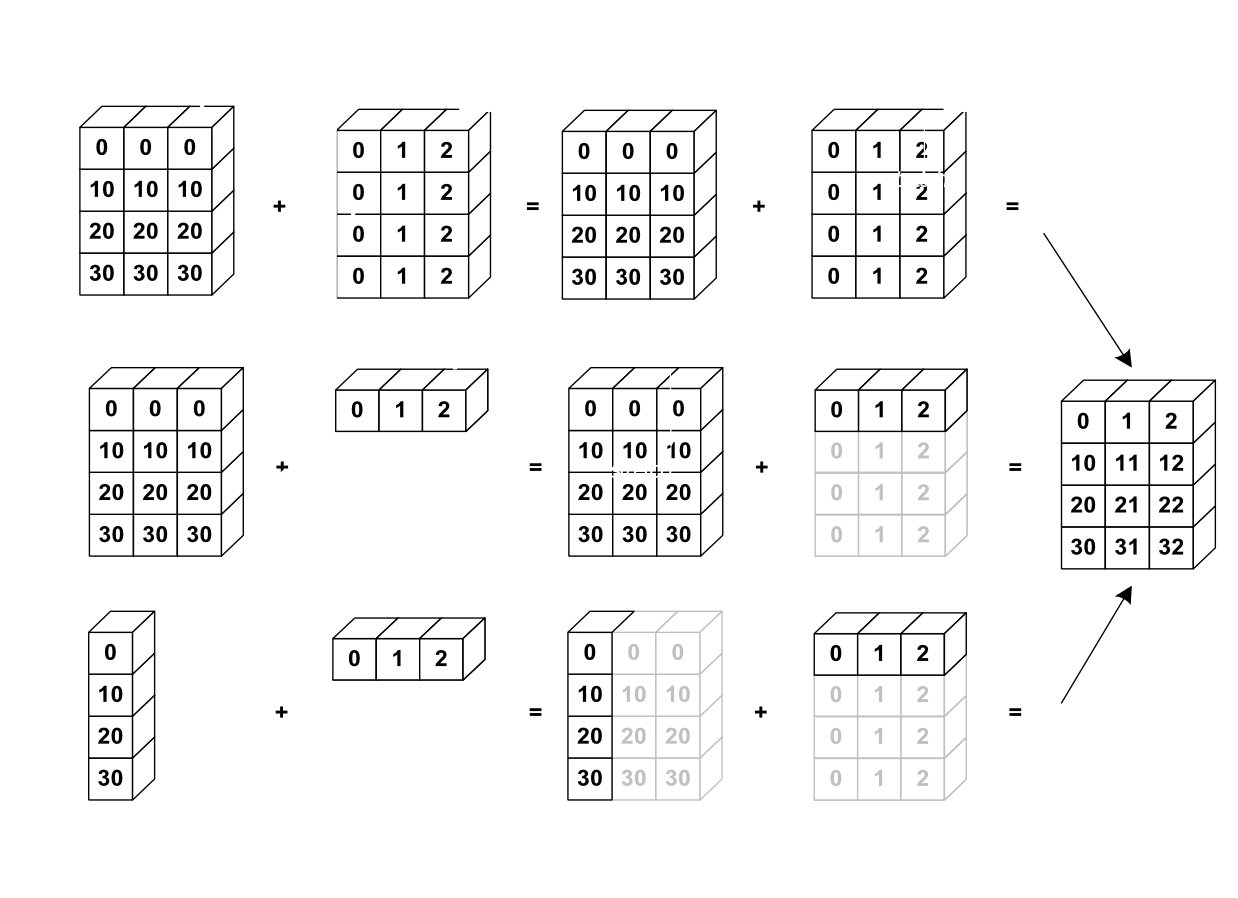
\includegraphics[height=2.5in]{broadcasting}
	\label{fig:xkcd}
	\end{subfigure}
\end{figure}
\end{frame}



\section{SciPy}

\begin{frame}
\frametitle{What is SciPy?}
SciPy is a library of algorithms and mathematical tools built to work with NumPy arrays.
\vspace{0.2in}
\begin{itemize}
\setlength{\itemsep}{0.1in}
\item{statistics - \textit{scipy.stats}}
\item{optimization - \textit{scipy.optimize}}
\item{sparse matrices - \textit{scipy.sparse}}
\item{signal processing - \textit{scipy.signal}}
\item{etc.}
\end{itemize}
\end{frame}


\begin{frame}
\frametitle{Example: KS-test}
Question: do two data samples come from the same distribution?
\lstset{basicstyle=\scriptsize}
\codeblock{code/ks_test.py}
\end{frame}

\begin{frame}
\lstset{basicstyle=\scriptsize}
\frametitle{Example: bootstrapped confidence interval}
\codeblock{code/bootstrap_mean.py}
\end{frame}

\begin{frame}
\frametitle{Example: k-Nearest Neighbor clustering}
\codeblock{code/knn.py}
\end{frame}

\end{document}
